\section{AEF-RPL: Proposed Approach}\label{sec:method}
\subsection{System and Threat Model}
The network uses RPL in non-storing mode, a common setup in constrained IIoT meshes in which only the root stores routes. Clients send one UDP packet to the root every 10~s, and the root returns it. Each packet thus crosses the network in both directions, and the measurements include upward damage from DIS floods as well as downward damage from false DAOs.

The adversary is an insider that controls some non-root nodes with valid credentials. RPL's optional security mode authenticates messages, but it cannot stop a key holder from sending well-formed malicious control messages \cite{rfc6550,raoof2019}, which is why we chose this model. Three attack modes were implemented. In DIS mode, the compromised node multicasts a DIS every 3~s by default. In DAO mode, it advertises its own prefix every 2~s and names a false transit parent, picked at random among the identifiers other than its own and its real parent's. The target and lifetime fields stay valid, so the DAO passes all format checks and its rate looks normal. Combined mode runs both from the same node. Every attack starts 300~s after boot (Fig.~\ref{fig:threat}). Root compromise, identity forgery, and jamming are out of scope, as they need authentication or physical-layer protection instead.

\begin{figure*}[t]
\centering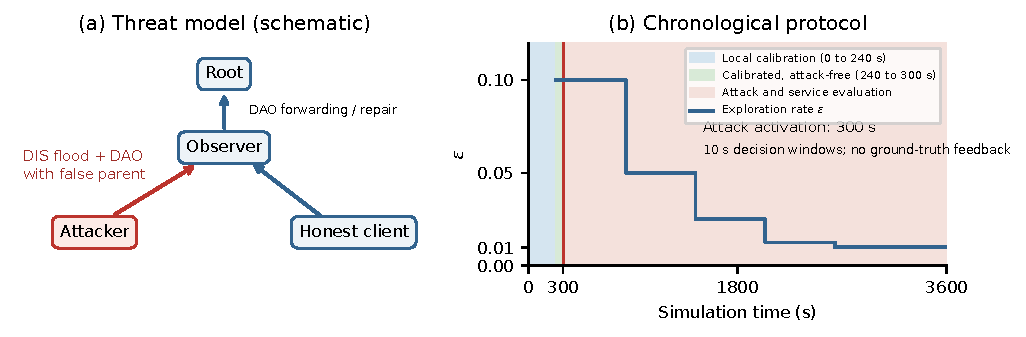
\includegraphics[width=.9\textwidth]{full_paper/generated/threat_timeline.pdf}
\caption{(a) The same compromised node floods DIS and sends DAOs with a false parent; an observer checks DAOs it receives directly from their originator and repairs them after isolation. (b) Time line of every 60-minute run: local calibration, then attack activation at 300~s.}\label{fig:threat}
\end{figure*}

\subsection{Local Observations and Self-Calibration}
Each node evaluates its neighbors once per decision window of $W=10$~s, the window length used by DIS-FDM \cite{prajisha2025}. Let $N_i(w)$ denote the IPv6 packets received by node $i$ in window $w$, and $D_{ij}(w)$ the DIS messages it received from neighbor $j$. The DIS indicator is $d_{ij}(w)=D_{ij}(w)/N_i(w)$, set to $0$ when $N_i(w)=0$. Rather than using a fixed threshold, each node derives its own from the first 240~s:
\begin{equation}
 \theta_i=\frac{1+\sum_w\sum_jD_{ij}(w)}{2+\sum_wN_i(w)}.
\end{equation}
With Laplace smoothing, this ratio is the posterior mean of the benign DIS share under a uniform prior. It follows the node's own traffic and stays defined when few packets were seen during calibration. A per-neighbor counter $c_D$ goes up by one in each window where $d_{ij}>\theta_i$, returns to zero otherwise, and saturates at five. Only consecutive exceedances count, which means that a single burst of legitimate solicitations (after a reboot, for instance) cannot lead to isolation. Two more counters come from DIS-FDM: $c_P$ for rapid preferred-parent changes over 60~s, and $c_E$ for radio and CPU activity above the calibration mean plus one standard deviation, with the statistics updated by Welford's method. The parent-change thresholds were obtained from attack-free calibration runs, 9.3~s for static and 16.5~s for mobile networks. Mobile networks get their own value because moving nodes change parents more often.

\subsection{DAO-Consistency Evidence}
A node in non-storing mode sends its DAO upward via its preferred parent and puts that parent in the transit-parent field \cite{rfc6550}. An observer $i$ that receives a DAO directly from the originator ($s=o$, nonzero lifetime) should therefore find itself named as the parent, $p=i$. If $p\neq i$, the observation counts as inconsistent. Only first-hop DAOs are checked, since a forwarded DAO legitimately names a parent other than the forwarder. The check uses an existing packet field and requires no keys or extra messages.

Honest nodes occasionally produce inconsistent DAOs too, for example while they switch parents, and the weight of this evidence has to reflect how often that happens. We therefore calibrate its uncertainty instead of fixing it (Gap~2). Let $F_i$ be the number of eligible DAOs that node $i$ observed during calibration and $B_i$ the number of inconsistent ones. Then
\begin{equation}
 \epsilon_i=\frac{B_i+1}{F_i+2}
\end{equation}
is the mean of the Beta reputation \cite{josang2002,ganeriwal2008}. In a network where honest DAOs are always consistent, $\epsilon_i$ approaches zero and the DAO evidence becomes strong, whereas a noisy network keeps it weak. Evidence is counted only after inconsistencies have appeared in two successive windows. From the second such window on, each window with an inconsistency adds the mass $(m(A),m(N),m(\Theta))=(1-\epsilon_i,0,\epsilon_i)$, and a clean window resets it. The choice of two windows comes from an ablation in which immediate evidence raised the static FPR from 11.8\% to 20.5\% (Section~\ref{sec:results}).

\subsection{Evidence Fusion and Decision}
On the frame $\Theta=\{A,N\}$ (attack, normal), the DIS, parent-change, and activity counters map to masses through DIS-FDM's tables: $0\mapsto(0,0,1)$, $1\mapsto(0,.8,.2)$, $2\mapsto(0,.6,.4)$, $3\mapsto(.6,0,.4)$, and $4,5\mapsto(.8,0,.2)$. They are fused with the DAO mass by Dempster's rule \cite{sentz2002}:
\begin{equation}
 (m_1\oplus m_2)(X)=\frac{\sum_{Y\cap Z=X}m_1(Y)m_2(Z)}{1-K},
\end{equation}
where $K=m_1(A)m_2(N)+m_1(N)m_2(A)$ measures conflict. We kept Dempster's rule, rather than a weighted average, because it lets agreeing sources reinforce each other while conflicting ones cancel, which suits independent views of one neighbor. When $K\ge.9999$, the node returns vacuous evidence instead of dividing by a near-zero term. The fixed decision keeps DIS-FDM's counter rules and adds one DAO rule: isolate when the fused $m(A)\ge\tau=.95$ and $m(A)>m(N)$. We set $\tau=.95$ at DIS-FDM's highest belief band, so that DAO evidence alone isolates a neighbor only when it is strong.

\subsection{Selective DAO Repair}
Isolation suppresses a neighbor's DIS processing, which stops the flood. For DAOs, the obvious response is to drop all of them, but this also removes the downward routes of the attacker's honest descendants, whose DAOs it forwards. AEF-RPL therefore lets an isolated originator's first DAO in each window pass and rewrites its false parent to the true one: the observer's own address on a forwarding path, or the DODAG identifier at the root. It updates the ICMPv6 checksum and drops any further DAOs in that window. The root then installs a correct source route. Section~\ref{sec:results} shows that this step accounts for most of the difference in downward service between AEF-RPL and DIS-FDM, although both detect the same attackers.

\subsection{On-Node Q-Learning Decision Layer}
Under the fixed rules, every node responds in the same way. To allow each node to adapt its response to local conditions (Gap~4), AEF-RPL hands the final accept/isolate choice to a tabular Q-learner \cite{watkins1992}. The evidence model stays the same, so differences from the fixed rule can be attributed to learning.

The learner's state $s=(c_D,b,\delta,\iota)$ consists of the DIS counter $c_D\in\{0,\dots,5\}$, the fused attack belief divided into four bins with edges at .5, .8, and .95 (the decision bands of DIS-FDM), a flag $\delta$ that marks current DAO evidence, and a flag $\iota$ that marks current isolation. This gives $6\times4\times2\times2=96$ states. Each node keeps a single table for all of its neighbors, so what it learns from one neighbor carries over to the others.

There are two actions, accept and isolate. For safety, two cases have a fixed action: a saturated DIS counter always leads to isolation, as in DIS-FDM's hard rule, and a state without any evidence always leads to acceptance. In the remaining states, a tie between the two values is resolved by the fixed rule, so an untrained learner behaves exactly like it.

Because no node knows which of its neighbors are attackers, the reward is based on a local anomaly indicator $z$ in the following window, namely a DIS threshold exceedance or a DAO inconsistency. With $z=0$ and $z=1$, accepting yields $0$ and $-1$, and isolating yields $-2$ and $+1$. A wrong isolation is penalized twice as much as a missed anomaly. The first cuts off an honest node's service, whereas a missed window can still be corrected one window later.

The table is updated after each window as
\begin{equation}
 Q(s,a)\leftarrow Q(s,a)+\alpha_{s,a}\big[r+\gamma\max_{a'}Q(s',a')-Q(s,a)\big],
\end{equation}
with $\alpha_{s,a}=1/\min(v_{s,a},16)$, where $v_{s,a}$ is the visit count, and $\gamma=.5$. For the first 16 visits the step size averages the samples, so the learner picks up quickly from an empty table. It then stays at $1/16$, which lets it follow a neighbor whose behavior changes. With this discount the horizon is roughly two windows, in line with the two-window persistence of the evidence, and $|Q|$ stays at most 4 (Section~\ref{sec:theory}). Exploration is $\varepsilon$-greedy. After calibration $\varepsilon=.10$, and it halves every 600~s down to .01, so most exploration takes place while the table is still empty. Two additional rules restrict it: exploration is allowed only in states with suspicious evidence or an active isolation, and an isolated neighbor is released only after two calm windows. Both keep random exploration from isolating neighbors that show no anomaly, and they are the only change to the decision layer specified in the research proposal. The artifact also contains a first version without these rules, which explored in every state and released a neighbor as soon as accept was chosen. Its false-positive rates were similar, but its policy was less stable. In the last 10 minutes of a mobile combined-attack run, up to 6.1 greedy actions changed per node, compared with 2.7 for the final version.

Values and rewards use Q8.8 fixed point, since many constrained microcontrollers have no floating-point unit. The Q-table and visit counts need $96\times2\times(2+2)=768$~bytes, and the policy bitmap needs 12 more.

Fig.~\ref{fig:algorithm} summarizes the per-window procedure.

\begin{figure}[t]
\centering\footnotesize
\fbox{\begin{minipage}{.95\columnwidth}
\textbf{Algorithm 1:} AEF-RPL at node $i$, every window $w$\\[2pt]
\begin{tabular}{@{}r@{\;}l@{}}
1:& \textbf{on} DIS from $j$: $D_{ij}\mathrel{+}=1$\\
2:& \textbf{on} DAO with origin $o$, sender $s$, parent $p$:\\
3:& \quad\textbf{if} $s=o$ \textbf{and} $p\neq i$ \textbf{then} mark DAO hit for $o$\\
4:& \quad\textbf{if} $o$ isolated: forward first DAO with $p\leftarrow$ true parent;\\
  & \quad\phantom{\textbf{if} $o$ isolated:} drop the rest of window $w$\\
5:& \textbf{at end of} $w$, \textbf{for each} active neighbor $j$:\\
6:& \quad \textbf{if} $t<240$\,s: update $\theta_i$, $\epsilon_i$, activity mean; \textbf{continue}\\
7:& \quad update $c_D$, $c_P$, $c_E$ and the DAO hit run\\
8:& \quad $m\leftarrow m_D\oplus m_P\oplus m_E\oplus m_{\mathrm{DAO}}$\\
9:& \quad $f\leftarrow$ fixed rule$(c_D,c_P,m)$\\
10:& \quad $s'\leftarrow(c_D,\mathrm{bin}(m(A)),\delta,\iota)$\\
11:& \quad $Q$-update for the previous $(s,a)$ with $r(a,z)$ and $s'$\\
12:& \quad $a\leftarrow$ safe $\varepsilon$-greedy$(s',f)$; apply isolate or release\\
13:& clear window counters; keep calibration and $Q$\\
\end{tabular}
\end{minipage}}
\caption{Per-window procedure of AEF-RPL. The learning-off ablation uses $a\leftarrow f$ in line~12.}\label{fig:algorithm}
\end{figure}
